% ========== DÅHJORT ==========
\begin{frame}{%
  \begin{minipage}[c]{0.30\textwidth}
    Dåhjort
  \end{minipage}%
  \hfill
  \begin{minipage}[c]{0.45\textwidth}
    \footnotesize
    \textbf{Jagttid:} 1.\ september -- 31.\ januar
  \end{minipage}%
  \hfill
  \begin{minipage}[c]{0.15\textwidth}
    \noindent\raggedleft
    
\includegraphics[width=0.5cm, height=0.5cm, keepaspectratio]{Billeder/Ikoner/star.png}%
    \hspace{0.2em}%
    
\includegraphics[width=0.5cm, height=0.5cm, keepaspectratio]{Billeder/Ikoner/star.png}%
    \hspace{0.2em}%
    
\includegraphics[width=0.5cm, height=0.5cm, keepaspectratio]{Billeder/Ikoner/star.png}
  \end{minipage}%
}
  \vspace{0.25em}
  \begin{columns}[T]
    \column{0.45\textwidth}
    \setlength{\parskip}{0.4em}
    \tiny
    \RaggedRight
    \textbf{\textit{Dama dama}} – næststørste hjorteart i Danmark. Hannen kaldes dåhjort og kendes på det skovlede (plade) gevir. I andet leveår kaldes den dåspidshjort. \par
    \textbf{Udseende:}\\
    \quad – Kort snudeskaft \\
    \quad – Hvidt spejl (111) \\
    \quad – Mange farvevariationer med pletter \par
    \textbf{Levesteder:} Skov, hegn og åbne landskaber. \par
    \textbf{Føde:} Græsser, urter, olden og landbrugsafgrøder. \par
    \textbf{Udbredelse:} Hele landet. \par
    \textbf{Parring/brunst:} Oktober/november. \par
    \textbf{Forplantning:}\\
    \quad – \textbf{Kønsmoden:} 1 år \\
    \quad – \textbf{Mono/polygam:} Polygam \\
    \quad – \textbf{Bestandsomsætning:} Langsom \\
    \quad – \textbf{Kuld:} 1 kalv, sjældent 2 \par
    %\textbf{*Bemærk:} Mange lokale jagttider.
    \column{0.52\textwidth}
    \centering
    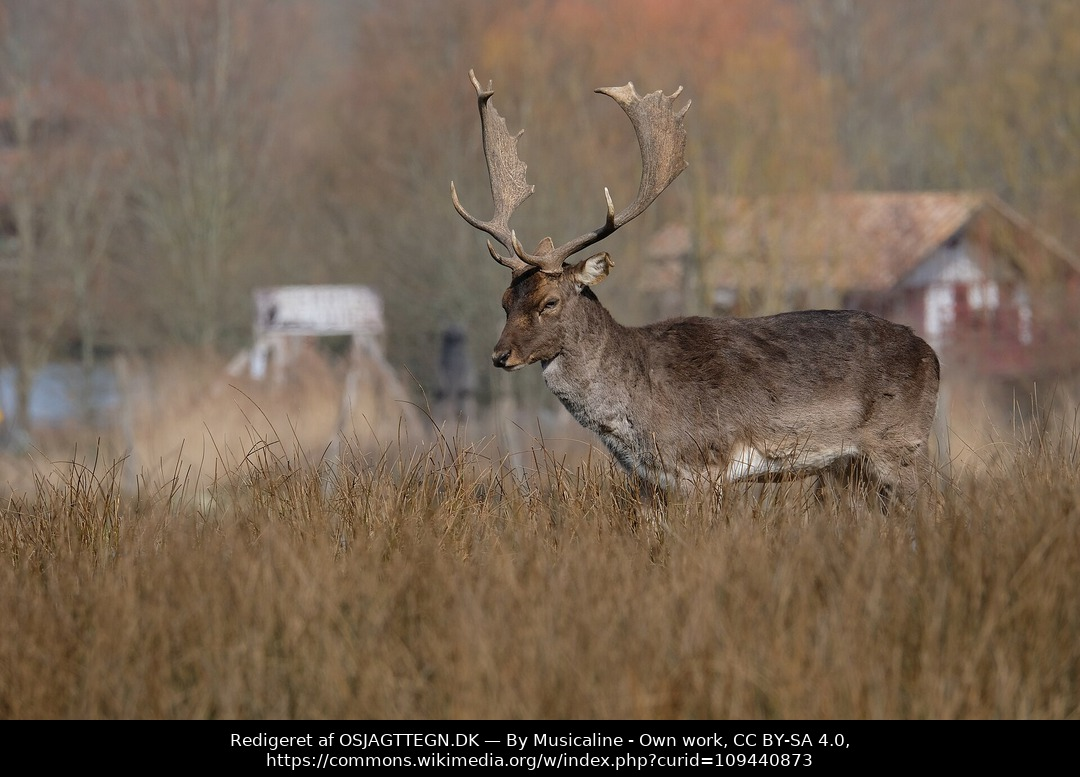
\includegraphics[width=\linewidth, height=7.2cm, keepaspectratio]{Billeder/Dyr/Pattedyr/hovdyr/dåvildt/daavildt-male-05.jpg}
  \end{columns}
\end{frame}